\chapter{System Validation: From Components to Scale}

% This chapter describes the metrics and procedures used to evaluate the effectiveness, efficiency, and usability of the proposed system. The evaluation is conducted at three levels: retriever, generator, and overall system performance.

\section{Evaluation}


\subsection{Document Parsing and Extraction Evaluation}

This section evaluates the quality of document parsing and structural extraction, which form the foundation of the entire RAG pipeline. Poor parsing quality leads to missing evidence, misaligned text blocks, and incorrect reading order-all of which degrade downstream retrieval and generation. We evaluate parsing across two comprehensive benchmarks: OmniDocBench for PDF documents and OfficeDocBench for office formats (DOCX, XLSX, PPTX).

\textbf{Evaluation Dataset Provenance and Scale}

To make the evaluation scope reproducible, Table~\ref{tab:evaluation_dataset_provenance} summarizes the source, scale, and evaluation role of each dataset used in this chapter. Public benchmark datasets are linked to their upstream sources, while the retrieval corpus is reported as an internally assembled local corpus because it is not a single public benchmark release.

\begin{table}[H]
    \centering
    \caption{Evaluation Dataset Provenance and Scale}
    \label{tab:evaluation_dataset_provenance}
    \scalebox{0.82}{
    \begin{tabular}{p{3.0cm}p{3.3cm}p{3.5cm}p{3.7cm}p{3.5cm}}
        \toprule
        \textbf{Dataset} & \textbf{Evaluation Role} & \textbf{Source} & \textbf{Documents / Units} & \textbf{Size} \\
        \midrule
        OmniDocBench & PDF parsing and structure extraction & \href{https://huggingface.co/datasets/opendatalab/OmniDocBench}{Hugging Face}; \href{https://github.com/opendatalab/OmniDocBench}{GitHub} & 1,650 annotated page images & $\sim$1.55 GB public dataset; $\sim$985 KB/page \\
        OfficeDocBench & Office document parsing benchmark & \href{https://www.sunholo.com/ailang-parse/benchmarks.html}{AILANG benchmark}; \href{https://github.com/sunholo-data/ailang-parse}{GitHub} & 43 files; DOCX pages, PPTX slides, XLSX sheets & Avg 31.4 KB; median 23.0 KB \\
        Pandoc DOCX/PPTX & Augmented Office-style parsing evaluation & \href{https://github.com/jgm/pandoc}{Pandoc GitHub} & 91 files; pages/slides & DOCX avg 20.2 KB; PPTX avg 33.0 KB \\
        DECO XLSX & Spreadsheet table/layout parsing evaluation & \href{https://tud.qucosa.de/en/landing-page/https\%3A\%2F\%2Ftud.qucosa.de\%2Fapi\%2Fqucosa\%253A82977\%2Fmets/}{DECO landing page} & 50 spreadsheets; sheets & Avg 242.1 KB; median 71.4 KB \\
        Retrieval PDF corpus & PDF QA/RAG retrieval evaluation & Local corpus & 100 PDF candidates; 43 selected-section files; 347 visual pages & Selected files avg 1,927.2 KB; range 65.5--16,805.9 KB \\
        \bottomrule
    \end{tabular}
    }
\end{table}

\textbf{Parsing Evaluation Protocol}

For parsing evaluation, the parser output is first converted into the same canonical schema as the benchmark ground truth. For OmniDocBench, each annotated page image is converted into ordered components such as text blocks, headings, tables, figures, and captions using the official \texttt{layout\_dets} annotations. For OfficeDocBench and the augmented Pandoc/DECO sets, parsed outputs are adapted into the OfficeDocBench flat schema containing fields such as \texttt{text\_elements}, \texttt{headings}, \texttt{tables}, \texttt{lists}, \texttt{comments}, \texttt{metadata}, and related structural features. Representative ground-truth formats are shown in Appendix~\ref{chap:evaluation_gt_formats}.

The PDF parsing score is computed as a weighted information-preservation score over metric groups. For an applicable group $g$ with score $s_g$ and weight $w_g$, the overall parsing score is:
\[
S_{\mathrm{parse}} = \dfrac{\sum_g w_g s_g}{\sum_g w_g}.
\]

The main groups are text fidelity, table extraction, read order, section hierarchy, and figure/caption association. 

Text fidelity uses token multiset precision and recall:

$$P=\dfrac{|T_{gt}\cap T_{pred}|}{|T_{pred}|}, \quad R=\dfrac{|T_{gt}\cap T_{pred}|}{|T_{gt}|}$$,

combined as $F_1=\dfrac{2PR}{P+R}$. 

Table quality combines detection coverage with content similarity: matched tables are scored using official OmniDocBench TEDS when available, otherwise a tree/edit fallback is used; the table group score is the average of coverage F1 and mean table-content score. Read order is pairwise order accuracy over matched components:
\[
S_{\mathrm{order}} = \dfrac{\#\{(i,j): \mathrm{order}_{gt}(i,j)=\mathrm{order}_{pred}(i,j)\}}{\#\{(i,j)\}}.
\]
Section hierarchy is computed as $0.6 \times$ node recall plus $0.4 \times$ path/level accuracy. OfficeDocBench uses its official composite formula: feature detection (15\%), structural recall (20\%), structural quality (15\%), content fidelity (15\%), text Jaccard (10\%), element-count accuracy (15\%), and metadata accuracy (10\%). 

The formula for calculating Text Jaccard is $\dfrac{|W_{gt}\cap W_{pred}|}{|W_{gt}\cup W_{pred}|}$.

\textbf{OmniDocBench Results}

OmniDocBench is a large-scale PDF parsing benchmark spanning 1,650 annotated pages with diverse document types including academic papers, books, presentations, exams, and magazines in both English and Chinese. The upstream dataset is available through Hugging Face and GitHub, with a public asset size of approximately 1.55 GB, or about 985 KB per annotated page. Exact local source-asset file-size statistics could not be recomputed because the raw OmniDocBench assets were not present in the local workspace. Each document is annotated with block-level and span-level categories, reading order, and table/formula structure. We evaluated \textbf{DocumentProcessorV2} in Hybrid Mode, which combines \textbf{ItemSequencer} (structural hierarchy using PyMuPDF) with \textbf{Docling} (text and table extraction with OCR enabled, VLM disabled).

\begin{table}[H]
    \centering
    \caption{OmniDocBench Parsing Evaluation (1650 Pages, DocumentProcessorV2 Hybrid).}
    \label{tab:omnidocbench_results}
    \scalebox{0.90}{
    \begin{tabular}{lrrrrr}
        \toprule
        \textbf{Metric} & \textbf{Score} & \textbf{Weight} & \textbf{Interpretation} \\
        \midrule
        \textbf{Overall Score} & 58.91\% & Combined & Strong foundation with identified bottleneck \\
        Read Order & 92.60\% & 15\% & Exceptional-preserves logical flow in complex layouts \\
        Table Score & 76.86\% & 25\% & Reliable table extraction with TEDS/grid accuracy \\
        Section Hierarchy & 90.14\% & 15\% & Excellent heading/structure preservation \\
        Text Score & 47.43\% & 30\% & Bottleneck-OCR and formula fidelity challenges \\
        \bottomrule
    \end{tabular}
    }
\end{table}

The results reveal a system that excels at structural tasks but struggles with text fidelity. The 92.60\% Read Order score demonstrates robust handling of multi-column layouts and complex document structures, proving the effectiveness of ItemSequencer's hierarchy approach. The 76.86\% Table Score shows that Docling's grid extraction is reliable even without vision-language models, correctly identifying cell boundaries and merged cells. However, the 47.43\% Text Score indicates that token-level extraction remains challenging, primarily due to missing complex LaTeX formulas, text block fragmentation on heavily mathematical pages, and OCR noise. The comparison is against OmniDocBench's page-level ground truth after both prediction and annotation are converted into the same canonical component schema; it is therefore a strict token-preservation measurement, not an end-user answer-quality score. In the reported run, \textbf{DocumentProcessorV2 Hybrid} uses ItemSequencer for structure and Docling with OCR enabled but VLM/formula enrichment disabled, so formula-heavy pages are expected to be the weakest case.

The low Text Score is mitigated downstream by the system's visual embedding pathway. Instead of relying only on OCR text, BK-MInD also rasterizes PDF pages and indexes them with ColQwen visual embeddings. This preserves page layout, formulas, diagrams, and table geometry as retrievable evidence even when the text parser cannot fully serialize them. Table~\ref{tab:ocr_vlm_tradeoff} summarizes the expected trade-off if formula/VLM extraction is enabled in future runs. The latency numbers are operational planning estimates rather than results included in the current benchmark, because the reported parsing score was produced with VLM disabled.

\begin{table}[H]
    \centering
    \caption{OCR-Only vs. VLM/Formula-Enriched Parsing Trade-off}
    \label{tab:ocr_vlm_tradeoff}
    \scalebox{0.86}{
    \begin{tabular}{p{3.6cm}p{4.4cm}p{4.0cm}p{3.5cm}}
        \toprule
        \textbf{Configuration} & \textbf{Expected Improvement} & \textbf{Main Trade-off} & \textbf{Latency Budget} \\
        \midrule
        OCR-only Docling path (current reported run) & Fast text extraction for paragraphs, headings, and many tables & Weak on math formulas, dense diagrams, and visual-heavy pages & Baseline; typically a few seconds per page depending on layout and hardware \\
        Selective VLM/formula enrichment & Better recovery of equations, formula-adjacent text, chart labels, and visual-heavy content & Higher GPU cost and slower ingestion; should be applied only to detected formula/visual pages & Plan for an additional $\sim$5--15 seconds per selected page on GPU-backed inference; CPU-only can be substantially slower \\
        Visual embedding pathway (current mitigation) & Retrieves the original rendered page even when OCR text is incomplete & Does not convert formulas into clean text; generator must read visual evidence & Indexing-time cost, but improves retrieval robustness for formula/layout evidence \\
        \bottomrule
    \end{tabular}
    }
\end{table}

% \textbf{OfficeDocBench Results}

% OfficeDocBench evaluates classical office document parsing across DOCX, XLSX, and PPTX formats. We evaluated 43 files (29 DOCX, 6 XLSX, 8 PPTX) representing the locally supported Office subset of the benchmark. The evaluation measures text preservation, structural recall, element accuracy, and feature detection across various document complexities.

% \begin{table}[H]
%     \centering
%     \caption{OfficeDocBench Results by Format}
%     \label{tab:officedocbench_results}
%     \scalebox{0.90}{
%     \begin{tabular}{lrrrrr}
%         \toprule
%         \textbf{Format} & \textbf{Files} & \textbf{Composite} & \textbf{Text Jaccard} & \textbf{Struct Recall} & \textbf{Feature Detect} \\
%         \midrule
%         DOCX & 29 & 60.98\% & 78.56\% & 67.80\% & High \\
%         PPTX & 8 & 54.10\% & Good & Moderate & Partial \\
%         XLSX & 6 & 43.10\% & Moderate & Lower & Lower \\
%         \bottomrule
%     \end{tabular}
%     }
% \end{table}

Office-based evaluation combines three source groups: OfficeDocBench, Pandoc DOCX/PPTX tests, and DECO spreadsheet files. Table~\ref{tab:office_dataset_scale} reports the dataset scale used for the Office-based parsing evaluations, while Table~\ref{tab:office_format_distribution} groups the same files by native format. Average units denote pages for DOCX files, slides for PPTX files, and sheets for XLSX files.

\begin{table}[H]
    \centering
    \caption{Office-Based Evaluation Dataset Scale}
    \label{tab:office_dataset_scale}
    \scalebox{0.88}{
    \begin{tabular}{lrrr}
        \toprule
        \textbf{Dataset Slice} & \textbf{Files} & \textbf{Avg Size (KB)} & \textbf{Avg Units (Page/Slide/Sheet)} \\
        \midrule
        OfficeDocBench & 43 & 31.4 & 1.61 \\
        Pandoc (DOCX/PPTX) & 91 & 22.8 & 1.42 \\
        DECO XLSX & 50 & 242.1 & 10.46 \\
        \bottomrule
    \end{tabular}
    }
\end{table}

\begin{table}[H]
    \centering
    \caption{Office-Based Evaluation Files by Format}
    \label{tab:office_format_distribution}
    \scalebox{0.88}{
    \begin{tabular}{lrrr}
        \toprule
        \textbf{Format} & \textbf{Files} & \textbf{Avg Size (KB)} & \textbf{Avg Units (Page/Slide/Sheet)} \\
        \midrule
        DOCX & 101 & 21.4 & 1.10 pages \\
        PPTX & 27 & 45.3 & 2.78 slides \\
        XLSX & 56 & 217.0 & 9.54 sheets \\
        \bottomrule
    \end{tabular}
    }
\end{table}

Across all formats, text extraction is strong at 78.56\% Jaccard overlap, indicating good word-level preservation. Structural recall of 67.80\% shows that most headings, tables, and lists are captured, though some complex structures like merged cells in spreadsheets are missed. Feature detection at 56.55\% indicates that basic features (headings, tables, comments) work well, but advanced features (bookmarks, track changes) are partially missed. Format-specific findings show that DOCX parsing is most mature (60.98\% composite), PPTX is moderate (54.10\%), and XLSX is challenging (43.10\%), reflecting the complexity of spreadsheet structure and merged cells.

These results confirm that the parsing pipeline successfully extracts the primary document content and structure needed for RAG applications. While perfect fidelity is unattainable due to inherent format differences and legacy document quirks, the achieved scores are sufficient for retrieval to locate relevant information. The parsing quality now sets the upper bound for all downstream retrieval and generation quality.

\subsection{Multimodal Retrieval Evaluation}

This section evaluates whether the system can reliably retrieve relevant text and visual evidence in response to user queries. Retrieval quality directly impacts answer correctness: if the right passages are not retrieved, the language model cannot generate correct answers even with perfect generation. We evaluate both text and image retrieval strategies, as well as media (video/audio) parsing quality.

\textbf{PDF Retrieval Benchmark Setup}

The updated PDF retrieval evaluation uses a larger benchmark designed to measure whether the retrieval layer can recover evidence from realistic academic and instructional documents. The corpus is stored locally under \texttt{backend/input/eval-input} and consists of educational PDF material assembled from course notes, lecture slides, assignments, readings, and textbooks. From 100 PDF candidates after filename filtering, we selected 43 files that are in English and under 100-page, with selected sections (over 1000 characters), 120 selected sections, and 600 generated questions. Each parsed eligible section generated five questions: three simple factual questions, one multi-intent question, and one reasoning question. This resulted in 360 simple questions, 120 multi-intent questions, and 120 reasoning questions. Retrieved evidence was judged using a graded relevance scale from 0 to 3, with strict binary relevance defined as relevance $\geq 2$ for Recall@K. nDCG@K uses the full graded relevance score and therefore measures ranking quality rather than only binary hit rate.

\begin{table}[H]
    \centering
    \caption{PDF Retrieval Evaluation Dataset}
    \label{tab:pdf_retrieval_dataset}
    \scalebox{0.88}{
    \begin{tabular}{lr}
        \toprule
        \textbf{Component} & \textbf{Count} \\
        \midrule
        PDF candidates & 100 \\
        English-filtered PDFs & 43 \\
        Selected sections & 120 \\
        Generated questions & 600 \\
        Simple questions & 360 \\
        Multi-intent questions & 120 \\
        Reasoning questions & 120 \\
        PDFs in visual database & 43 \\
        Embedded visual pages & 347 \\
        \bottomrule
    \end{tabular}
    }
\end{table}

The selected retrieval files range from small assignment PDFs to larger technical books. Table~\ref{tab:pdf_retrieval_size_stats} reports file-size statistics in kilobytes for the selected files used to generate questions. The visual index embeds 347 rendered pages from 43 PDFs.

\begin{table}[H]
    \centering
    \caption{Selected PDF Retrieval File Size Statistics}
    \label{tab:pdf_retrieval_size_stats}
    \scalebox{0.88}{
    \begin{tabular}{lr}
        \toprule
        \textbf{Statistic} & \textbf{Size (KB)} \\
        \midrule
        Minimum & 65.5 \\
        Median & 959.5 \\
        Average & 1,927.2 \\
        Maximum & 16,805.9 \\
        \bottomrule
    \end{tabular}
    }
\end{table}

\begin{table}[H]
    \centering
    \caption{Retrieval Corpus Source Distribution}
    \label{tab:retrieval_source_distribution}
    \scalebox{0.86}{
    \begin{tabular}{p{8.6cm}rrr}
        \toprule
        \textbf{Source Folder} & \textbf{Selected Files} & \textbf{Selected Sections} & \textbf{Questions} \\
        \midrule
        \texttt{CS131 Notes zh-CN} & 11 & 45 & 225 \\
        \texttt{CS228 PGM} & 3 & 44 & 220 \\
        \texttt{Stanford University Algorithms Design \& Analysis} & 20 & 20 & 100 \\
        \texttt{CS193P Fall 2017 DEMO} & 9 & 11 & 55 \\
        \bottomrule
    \end{tabular}
    }
\end{table}

The retrieval run completed without retrieve-stage failures: 600 text-retrieval questions and 600 visual-retrieval questions were judged, with zero text or visual retrieve errors recorded in the evaluation artifacts.

\textbf{Coverage Proof}

The benchmark is intentionally section-driven rather than manually cherry-picked. After English and parseability filters, every parsed section that passed the minimum-content rule was eligible for question generation. The coverage is therefore conditional on sections that the system could parse into usable evidence, which is the correct scope for evaluating the retrieval layer. Table~\ref{tab:qa_coverage_proof} summarizes this coverage across documents, sections, modalities, and question types.

\begin{table}[H]
    \centering
    \caption{Question Set Coverage Proof}
    \label{tab:qa_coverage_proof}
    \scalebox{0.84}{
    \begin{tabular}{p{3.2cm}p{5.2cm}p{4.6cm}p{3.8cm}}
        \toprule
        \textbf{Coverage Axis} & \textbf{Retrieval Evaluation} & \textbf{End-to-End Evaluation} & \textbf{Control Mechanism} \\
        \midrule
        Documents & 43 English, parseable PDF files from the local educational corpus & 20 documents used for complete retrieval-generation judging & Filename/content language filtering and parse-success filtering \\
        Sections & 120 selected parsed sections & 132 selected parsed sections & Minimum section length; short, boilerplate, and table-of-contents-like sections excluded \\
        Questions per section & Exactly 5 questions per section & Exactly 5 questions per section & Fixed generator contract, not arbitrary sampling \\
        Question types & 360 simple, 120 multi-intent, 120 reasoning & Same section-based generation pattern & Type-balanced template: 3 simple + 1 multi-intent + 1 reasoning \\
        Modalities / evidence units & Text chunks and visual PDF pages are both evaluated & Retrieved context is judged for final answer support & Each item stores source document, section id, heading breadcrumb, reference answer, and evidence hint \\
        Task coverage & Retrieval-only quality via Recall@K and nDCG@K & Full RAG quality via correctness, faithfulness, and answer support & Separate metrics diagnose retrieval ranking vs. answer generation \\
        \bottomrule
    \end{tabular}
    }
\end{table}

\textbf{PDF Retrieval Evaluation Protocol}

The PDF retrieval benchmark follows a staged pipeline: discover candidate PDFs, remove obvious non-English filenames, parse each PDF into section-aware text artifacts, apply an English-content filter, select valid sections, generate synthetic questions, build text and visual indexes, retrieve top-10 evidence, and judge evidence relevance with an LLM. A PDF passes the content filter when it contains at least 500 Latin alphabetic characters and has a CJK character ratio below 0.05. A section is eligible when it has enough substantive content, is not boilerplate (e.g., declaration, preface, acknowledgements), and is not table-of-contents-like. This removes cases where a generated question would only test a title, a page number, or metadata instead of recoverable evidence.

Question generation is performed section by section using \texttt{zai-glm-4.7-flash} through AWS Bedrock. Each selected section produces exactly five questions using only the source section: three \texttt{simple} questions, one \texttt{multi\_intent} question, and one \texttt{reasoning} question. Generated questions are admitted only when the reference answer and expected evidence can be grounded in the same source section. Items are rejected or regenerated if they are malformed, duplicate another question from the same section, answerable only from the section title, too vague, or not supported by a clear evidence hint. Each accepted item stores the question, reference answer, expected evidence hint, source document, section id, heading, breadcrumb, and question type. The detailed record format is shown in Appendix~\ref{chap:evaluation_gt_formats}. Text retrieval uses a hybrid score,
\[
\mathrm{score}_{hybrid}=0.5 \cdot \mathrm{cosine}(q,d)+0.5 \cdot \mathrm{BM25}_{norm}(q,d),
\]
where dense embeddings are generated with \texttt{all-MiniLM-L6-v2} and BM25 scores are min-max normalized. Visual retrieval renders each indexed PDF page as an image and embeds pages with \texttt{vidore/colqwen2-v1.0}; the evidence unit is therefore a full PDF page rather than a text chunk.

The relevance judge uses \texttt{gpt-5.4-nano}. It receives the question, reference answer, expected evidence hint, and the retrieved evidence list. For visual evidence, the rendered page images are attached to the judge request. Each evidence item is assigned a relevance score in $\{0,1,2,3\}$: 0 = irrelevant, 1 = same topic but insufficient, 2 = partially answers the question, and 3 = highly relevant and sufficient. The report uses strict binary relevance $rel(e)=1$ when the judge score is at least 2. For query $q$, the strict Recall@K is:
\[
\mathrm{Recall@K}(q)=\dfrac{|\{e \in \mathrm{TopK}(q): rel(e)=1\}|}{|\{e: rel(e)=1\}|}.
\]
Ranking quality is measured with graded nDCG using the raw 0--3 relevance scores:
\[
\mathrm{DCG@K}=\sum_{i=1}^{K}\dfrac{2^{r_i}-1}{\log_2(i+1)},\qquad
\mathrm{nDCG@K}=\dfrac{\mathrm{DCG@K}}{\mathrm{IDCG@K}},
\]
where $r_i$ is the judged relevance at rank $i$ and IDCG is the best possible DCG for the same judged evidence set.

\textbf{Hybrid Text Retrieval Results}

Text retrieval was evaluated using the production hybrid retriever rather than isolated BM25-only or dense-only variants. The hybrid index combines BM25Okapi and SentenceTransformer dense retrieval using equal weighting: \texttt{hybrid\_score = 0.5 * dense\_score + 0.5 * normalized\_BM25\_score}. Dense retrieval uses \texttt{all-MiniLM-L6-v2}, while BM25 scores are min-max normalized before fusion.

\begin{table}[H]
    \centering
    \caption{Hybrid Text Retrieval Performance on PDF Dataset (n = 600)}
    \label{tab:hybrid_text_pdf_retrieval}
    \scalebox{0.88}{
    \begin{tabular}{lrrrr}
        \toprule
        \textbf{Metric} & \textbf{@1} & \textbf{@3} & \textbf{@5} & \textbf{@10} \\
        \midrule
        Recall & 38.07\% & 62.69\% & 75.85\% & \textbf{93.69\%} \\
        nDCG & 56.20\% & 61.55\% & 67.26\% & \textbf{73.83\%} \\
        \bottomrule
    \end{tabular}
    }
\end{table}

Hybrid text retrieval achieves strong candidate coverage at K=10, with Recall@10 reaching 93.69\%. This indicates that relevant evidence is usually present somewhere in the top-10 candidate set. However, Recall@1 is substantially lower at 38.07\%, showing that the main limitation is top-rank ordering rather than complete retrieval failure. In practical RAG terms, the text retriever is effective for constructing a broad evidence pool, but answer quality remains sensitive to reranking and context selection.

\textbf{Visual Retrieval Results}

Visual retrieval was evaluated using rendered PDF pages as the retrieval unit. Each page is embedded using \texttt{vidore/colqwen2-v1.0}, a ColQwen page-level multi-vector retriever designed for matching text queries against document page images. The current visual database contains 40 PDFs and 347 embedded pages.

\begin{table}[H]
    \centering
    \caption{Visual Retrieval Performance on PDF Dataset}
    \label{tab:visual_pdf_retrieval}
    \scalebox{0.88}{
    \begin{tabular}{lrrrr}
        \toprule
        \textbf{Metric} & \textbf{@1} & \textbf{@3} & \textbf{@5} & \textbf{@10} \\
        \midrule
        Recall & 63.06\% & 86.67\% & 91.12\% & \textbf{95.66\%} \\
        nDCG & 81.07\% & 84.98\% & 86.76\% & \textbf{88.91\%} \\
        \bottomrule
    \end{tabular}
    }
\end{table}

Visual retrieval outperforms hybrid text retrieval across all evaluated depths. The largest gains appear at the top of the ranking: Recall@1 improves from 38.07\% to 63.06\%, and nDCG@1 improves from 56.20\% to 81.07\%. This suggests that page-level visual retrieval not only recovers relevant evidence, but also places highly relevant evidence earlier in the ranking.

\textbf{Hybrid Text vs. Visual Retrieval Comparison}

\begin{table}[H]
    \centering
    \caption{Hybrid Text and Visual Retrieval Comparison}
    \label{tab:hybrid_text_visual_comparison}
    \scalebox{0.88}{
    \begin{tabular}{lrrr}
        \toprule
        \textbf{Metric} & \textbf{Hybrid Text} & \textbf{Visual} & \textbf{Difference} \\
        \midrule
        Recall@1 & 38.07\% & 63.06\% & +24.99\% \\
        Recall@3 & 62.69\% & 86.67\% & +23.98\% \\
        Recall@5 & 75.85\% & 91.12\% & +15.27\% \\
        Recall@10 & 93.69\% & 95.66\% & +1.96\% \\
        \midrule
        nDCG@1 & 56.20\% & 81.07\% & +24.87\% \\
        nDCG@3 & 61.55\% & 84.98\% & +23.44\% \\
        nDCG@5 & 67.26\% & 86.76\% & +19.49\% \\
        nDCG@10 & 73.83\% & 88.91\% & +15.07\% \\
        \bottomrule
    \end{tabular}
    }
\end{table}

The comparison changes the interpretation of PDF retrieval quality. Visual retrieval is currently the stronger modality for top-ranked PDF evidence, particularly at K=1 and K=3. This result is consistent with the nature of the dataset, which contains lecture notes, slides, mathematical notation, diagrams, tables, captions, and layout-dependent explanations. Rendered pages preserve heading context, visual grouping, formula placement, and table structure, whereas text retrieval depends on parsing and chunking decisions that may split a logically coherent page or section into several fragments. Hybrid text retrieval remains important because its Recall@10 is high, making it useful for candidate expansion and fallback evidence. However, improving text retrieval should focus on ranking quality, page-aware or section-aware chunking, heading breadcrumb preservation, and reranking rather than only increasing candidate depth.

\textbf{Question-Type Breakdown}

\begin{table}[H]
    \centering
    \caption{Retrieval Performance by Question Type}
    \label{tab:retrieval_by_question_type}
    \scalebox{0.86}{
    \begin{tabular}{llrrrr}
        \toprule
        \textbf{Modality} & \textbf{Question Type} & \textbf{Count} & \textbf{Recall@1} & \textbf{Recall@10} & \textbf{nDCG@10} \\
        \midrule
        Hybrid Text & Simple & 360 & 38.62\% & 92.82\% & 73.16\% \\
        Hybrid Text & Multi-intent & 120 & 30.17\% & 96.39\% & 69.59\% \\
        Hybrid Text & Reasoning & 120 & 44.35\% & 93.61\% & 80.10\% \\
        \midrule
        Visual & Simple & 228 & 62.51\% & 95.18\% & 87.44\% \\
        Visual & Multi-intent & 76 & 62.72\% & 96.05\% & 90.94\% \\
        Visual & Reasoning & 76 & 65.08\% & 96.71\% & 91.26\% \\
        \bottomrule
    \end{tabular}
    }
\end{table}

The question-type breakdown shows that multi-intent questions are the most difficult case for hybrid text retrieval at top-1, with Recall@1 of 30.17\%. This is expected because multi-intent questions often require evidence distributed across multiple local contexts, making chunk-level ranking more fragile. Visual retrieval is more stable across all three question types, with Recall@1 consistently above 62\% and nDCG@10 above 87\%. These results reinforce the role of page-level visual retrieval as the strongest evidence retriever for PDF QA in the current benchmark.

\textbf{Media Evaluation Protocol}

Media evaluation measures whether lecture video/audio can be converted into retrieval-ready temporal evidence. The pipeline extracts audio, transcribes speech with Whisper ASR, chunks the transcript by time span, and samples video frames at fixed intervals. ASR quality is measured using word error rate and character error rate:
\[
\mathrm{WER}=\dfrac{S_w+D_w+I_w}{N_w},\qquad
\mathrm{CER}=\dfrac{S_c+D_c+I_c}{N_c},
\]
where $S$, $D$, and $I$ denote substitutions, deletions, and insertions against the reference transcript, and $N$ is the number of reference words or characters. Temporal chunk quality is measured by hit rate and intersection-over-union (IoU). A chunk is a hit if it overlaps the gold time window; temporal IoU is $\mathrm{overlap}(t_{pred},t_{gt})/\mathrm{union}(t_{pred},t_{gt})$. Frame alignment is evaluated by checking whether each retrieved transcript chunk has an attached frame close to the target timestamp, including a tolerance-based variant within $\pm 2$ seconds.

\textbf{Media (Video/Audio) Evaluation}

Media parsing was evaluated on 42 MIT lecture videos (MITFLD subset, under 100MB each). The system performed four steps: (1) extracted audio from videos, (2) transcribed it using Whisper (speech-to-text), (3) split transcriptions into time-aligned chunks, and (4) sampled video frames every 100 frames to index visual content.

\begin{table}[H]
    \centering
    \caption{Media Parsing Quality Metrics (42 Lecture Videos).}
    \label{tab:media_results}
    \begin{adjustbox}{max width=\linewidth}
    \begin{tabular}{lrr}
        \toprule
        \textbf{Metric} & \textbf{Value} & \textbf{Interpretation} \\
        \midrule
        Mean WER (Word Error Rate) & 16.63\% & Percentage of incorrectly transcribed words \\
        Mean CER (Character Error Rate) & 11.26\% & Reliable character-level transcription \\
        Temporal Hit Rate & 100.0\%\footnotemark & All gold windows matched in chunks \\
        Temporal IoU & 34.84\% & Chunks align with expected time windows \\
        Frames Extracted & 12,020 & 285 frames per video (manageable) \\
        Frame Hit Rate & 97.65\%--100.0\% & Frames correctly attached to chunks \\
        \bottomrule
    \end{tabular}
\end{adjustbox}
\end{table}
\footnotetext{Temporal Hit Rate measures chunk recall (whether any chunk overlaps the target time window). Temporal IoU (34.84\%) measures precision (tightness of boundaries). The 100\% hit rate reflects excellent coverage; the 34.84\% IoU indicates chunks often span broader windows than necessary, acceptable for retrieval but limiting for sub-minute precision.}

ASR quality is good: 16.63\% WER (word error rate) is typical for Whisper tiny on CPU and acceptable for educational lecture retrieval. Temporal coverage is excellent (100\% hit rate for chunk recall), though temporal precision is moderate (34.84\% Temporal IoU), meaning chunks often span broader time windows than the exact target-acceptable for content retrieval but limiting for sub-minute precision seeking. Frame extraction succeeded on all 42 videos with proper timestamp metadata, enabling visual-temporal retrieval for video content.

% \textbf{OCW Single-Lecture Media Evaluation}

% To validate generalization beyond the MITFLD benchmark, media evaluation was conducted on a single MIT OpenCourseWare lecture from an alternative source. This evaluation provides comparative insights into ASR quality and temporal alignment across different audio conditions.

% \begin{table}[H]
%     \centering
%     \caption{OCW vs. MITFLD Media Evaluation Comparison.}
%     \label{tab:ocw_mitfld_comparison}
%     \scalebox{0.90}{
%     \begin{tabular}{lrrr}
%         \toprule
%         \textbf{Metric} & \textbf{MITFLD (42 videos)} & \textbf{OCW (1 video)} & \textbf{Interpretation} \\
%         \midrule
%         Mean WER & 16.63\% & 21.81\% & OCW audio lower clarity \\
%         Mean CER & 11.26\% & 17.38\% & Reflects higher WER \\
%         Temporal Hit Rate & 100.00\% & 100.00\% & Both achieve perfect coverage \\
%         Mean Temporal IoU & 34.84\% & \textbf{56.59\%} & OCW has tighter boundaries \\
%         \bottomrule
%     \end{tabular}
%     }
% \end{table}

% The OCW evaluation reveals an interesting trade-off: while the audio has lower clarity (21.81\% WER vs 16.63\%), temporal alignment is substantially tighter (56.59\% IoU vs 34.84\%). This suggests clearer fragment boundaries in the OCW lecture's transcript structure, despite noisier audio. Both sources maintain 100\% temporal hit rate, confirming that the chunking strategy reliably captures all gold windows regardless of audio quality variation. This validates that the media pipeline is robust across different lecture sources and audio conditions.

\textbf{Frame Extraction and Alignment Validation}

Beyond ASR and temporal metrics, the system extracts frames from video content and validates their temporal alignment with transcript chunks. This subsection reports frame extraction pipeline statistics and weak-supervised frame alignment metrics.

% \textbf{Frame Extraction Pipeline Statistics}

\begin{table}[H]
    \centering
    \caption{Frame Extraction and Processing Pipeline (42 Videos).}
    \label{tab:frame_extraction_stats}
    \scalebox{0.88}{
    \begin{tabular}{lrr}
        \toprule
        \textbf{Component} & \textbf{Count} & \textbf{Status} \\
        \midrule
        Input videos & 42 & All MITFLD videos \\
        Processed files & 42 & 100\% success rate \\
        Audio extracted & 42 & All successful \\
        Transcribed & 42 & All transcribed \\
        Transcript chunks & 3,072 & Temporal chunking complete \\
        Frames extracted & 12,020 & 100-frame interval \\
        Frame deduplication & Enabled & Reduced redundant frames \\
        Stage 4 rag-ready docs & 42 & All documents prepared \\
        Docs with chunks & 42 & 100\% coverage \\
        Docs with frames & 42 & 100\% coverage \\
        \bottomrule
    \end{tabular}
    }
\end{table}

The frame extraction pipeline processed all 42 videos without failures, extracting 12,020 frames (approximately 285 frames per video, manageable for indexing). All processed documents have both transcript chunks and frames attached, enabling visual-temporal retrieval downstream.

\textbf{Frame Alignment Metrics (Full MITFLD: 42 videos, 298 evaluation items)}

\begin{table}[H]
    \centering
    \caption{Frame Alignment Quality Across Retrieval Depths.}
    \label{tab:frame_alignment}
    \scalebox{0.88}{
    \begin{tabular}{lrrrr}
        \toprule
        \textbf{Metric} & \textbf{@1} & \textbf{@3} & \textbf{@5} & \textbf{@10} \\
        \midrule
        Chunk Hit & 100\% & 100\% & 100\% & 100\% \\
        Best Chunk IoU & 18.49\% & 21.70\% & 22.10\% & 22.58\% \\
        Chunk Temporal Recall & 20.52\% & 32.94\% & 38.27\% & 46.55\% \\
        Frame Hit & 97.65\% & 98.32\% & 98.32\% & 98.32\% \\
        \bottomrule
    \end{tabular}
    }
\end{table}

Frame alignment shows excellent attachment quality: 100\% chunk hit rate indicates that all retrieved chunks overlap the target time window, and frame attachment reaches 97.65\%--98.32\% coverage across retrieval depths. The 22.58\% Best Chunk IoU at @10 indicates moderate boundary tightness. This validates that the frame extraction pipeline successfully attaches visual content to transcript chunks with high fidelity.

\subsection{System-Level (End-to-end) Evaluation}

% This section measures end-to-end RAG quality from question to final answer.

% \textbf{Chunking Evaluation Protocol}

% Chunking evaluation uses span-level ground truth generated from the canonical stage-4 markdown corpus. Source documents are segmented into eligible excerpts, an LLM generates factual search queries from each excerpt, and each generated \texttt{relevant\_excerpt} must be verified as an exact contiguous substring of the source document before it is admitted into the evaluation set. Each ground-truth row therefore contains a query, source document id, relevant excerpt, and exact \texttt{start\_char}/\texttt{end\_char} offsets. The ground-truth row format is shown in Appendix~\ref{chap:evaluation_gt_formats}.

% For a retrieved top-K set, the evaluator maps each retrieved chunk back to one or more source character intervals. Let $G$ be the gold interval, $R_K$ be the union of retrieved intervals from the same source document, and $|\,\cdot\,|$ denote character length. The metrics are:
% \[
% \mathrm{Hit@K}=\mathbb{1}\{|R_K\cap G|>0\},\qquad
% \mathrm{SpanRecall@K}=\dfrac{|R_K\cap G|}{|G|},
% \]
% \[
% \mathrm{SpanPrecision@K}=\dfrac{|R_K\cap G|}{|R_K|},\qquad
% \mathrm{SpanIoU@K}=\dfrac{|R_K\cap G|}{|R_K\cup G|}.
% \]
% This evaluates whether a chunking strategy retrieves the exact source span needed to answer the query, while also penalizing overly broad chunks that include excessive irrelevant context.

% \textbf{Chunking Strategy Evaluation}

% Document chunking determines whether a retriever finds the exact passage needed to answer a question, or must sift through irrelevant neighbors. We compared two strategies on 111 synthetic query-span pairs from 3 documents (434K characters total): recursive markdown chunking (production baseline) and semantic cluster chunking (research variant).

% \begin{table}[H]
%     \centering
%     \caption{Chunking Quality: Recursive vs. Semantic (111 Queries)}
%     \label{tab:chunking_results}
%     \scalebox{0.90}{
%     \begin{tabular}{lrrrr}
%         \toprule
%         \textbf{Strategy} & \textbf{Hit@1} & \textbf{Span Recall@1} & \textbf{Span IoU@1} & \textbf{Avg Chars} \\
%         \midrule
%         Recursive Markdown & 72.07\% & 69.43\% & 18.71\% & 755 \\
%         Semantic Cluster & 72.97\% & 71.07\% & 15.89\% & 1,006 \\
%         \textbf{Winner (Tie)} & \textbf{Semantic} & \textbf{Semantic} & \textbf{Recursive} & \textbf{Recursive} \\
%         \bottomrule
%     \end{tabular}
%     }
% \end{table}

% Both strategies achieve similar hit rates (72\%). Semantic chunking provides slightly better recall (71.07\% vs 69.43\%), recovering more of the target span. However, recursive chunking achieves better precision (18.71\% vs 15.89\% IoU) because it retrieves fewer irrelevant characters, improving LLM efficiency. Semantic chunking retrieves approximately 33\% more average characters per chunk (1,006 vs 755), making recursive chunking more cost-efficient for generation. The production pipeline uses recursive chunking for its balance of simplicity and precision; semantic chunking remains a research direction for improving recall on long-answer questions.

\textbf{End-to-End RAG Evaluation Protocol}

End-to-end evaluation tests the complete question-answering path rather than retrieval alone. The pipeline follows the same section-grounded question generation methodology as the retrieval benchmark: it selects parsed English sections with sufficient content, generates factual question/reference-answer pairs with \texttt{zai-glm-4.7-flash} through AWS Bedrock using only that section as source material, and retains only questions whose answer can be traced to explicit source evidence. The local corpus is then indexed, evidence is retrieved with the configured RAG retriever, an answer is generated, and the question, reference answer, retrieved context, and generated answer are sent to the \texttt{gpt-5.4-nano} judge. The judge returns three categorical labels: \textbf{correctness}, \textbf{faithfulness}, and \textbf{answer\_support}.

% The reported rates are macro proportions over all evaluated questions. For a label set $L$ and target label $\ell$, the rate is:
% \[
% \mathrm{Rate}(\ell)=\dfrac{|\{q: \mathrm{judge}(q)=\ell\}|}{|\{q: q\ \mathrm{was\ evaluated}\}|}.
% \]

Correctness measures agreement with the reference answer, while faithfulness measures whether the answer is grounded in the retrieved context, and answer support measures whether the retrieved context itself contains enough evidence to justify the answer. This separation is important because an incorrect answer can be caused by missing retrieval evidence even when the generator remains faithful to the context it received.

\textbf{End-to-End Evaluation Results}

End-to-end evaluation measures complete system correctness: retrieval + generation + answer quality. We generated 660 questions from 132 sections across 20 documents, then evaluated answers on three dimensions: correctness (factual accuracy), faithfulness (grounding in retrieved context), and answer support (whether retrieval provided sufficient information).

\begin{table}[H]
    \centering
    \caption{End-to-End RAG Evaluation Results (660 Questions).}
    \label{tab:e2e_results}
    \begin{adjustbox}{max width=\linewidth}
    \begin{tabular}{lrr}
        \toprule
        \textbf{Dimension} & \textbf{Metric} & \textbf{Rate} \\
        \midrule
        \multirow{3}{*}{\textbf{Correctness}} & Correct & 72.7\% \\
        & Partially Correct & 4.8\% \\
        & Incorrect & 22.4\% \\
        \midrule
        \multirow{3}{*}{\textbf{Faithfulness}} & Faithful & 99.5\% \\
        & Partially Faithful & 0.5\% \\
        & Hallucinated & 0.0\% \\
        \midrule
        \multirow{3}{*}{\textbf{Answer Support}} & Fully Supported & 82.0\% \\
        & Partially Supported & 1.7\% \\
        & Not Supported & 16.4\% \\
        \bottomrule
    \end{tabular}
    \end{adjustbox}
\end{table}

The system achieves 72.7\% correctness, meaning answers are factually accurate for most questions. Critically, faithfulness reaches 99.5\% with zero hallucinations, indicating that the RAG pipeline is highly reliable and grounded in retrieved evidence. This high faithfulness-to-correctness ratio (99.5\% vs 72.7\%) reveals that most errors come from retrieval failures or incomplete context (16.4\% of answers lack full support) rather than generation failing to ground answers. This diagnosis suggests that improving retrieval quality and chunking precision will directly lift correctness toward higher levels.

The 82\% fully-supported rate confirms that the retrieval system successfully locates relevant passages for most queries, validating the combination of parsing, chunking, and retrieval strategies. The 22.4\% incorrect rate is primarily driven by questions whose answers require information not retrieved (16.4\%) or only partially retrieved (1.7\%), indicating retrieval as the primary optimization target for future improvements.

% \subsection{Evaluation Summary and Readiness Assessment}
% The comprehensive evaluation across document parsing, multimodal retrieval, chunking strategy, and end-to-end RAG generation establishes that the BK-MInD system achieves \textbf{high-quality component-level performance} with clear diagnostic insights for production readiness.

% \textbf{Key Findings:}

% \textit{(1) Parsing Quality Establishes Foundation-Strength in Structure, Bottleneck in Text Fidelity.} OmniDocBench parsing reaches 58.91\% overall accuracy, with exceptional read-order preservation (92.60\%) and strong table extraction (76.86\%), but text-level extraction lags at 47.43\% due to formula complexity and OCR limitations. Office document parsing (DOCX: 60.98\%) significantly outperforms spreadsheets (XLSX: 43.10\%), reflecting the structural complexity of merged cells and formula content. These results confirm that the parsing pipeline sets the upper bound for all downstream retrieval and generation quality.

\textit{(2) Visual Retrieval Provides Stronger Top-Ranked PDF Evidence, while Hybrid Text Maintains High Candidate Coverage.} On the updated PDF retrieval benchmark, hybrid text retrieval reaches strong Recall@10 (93.69\%), confirming that relevant evidence is usually present in the top-10 candidate pool. However, visual page-level retrieval with ColQwen performs better across all measured depths, reaching 95.66\% Recall@10 and 88.91\% nDCG@10, compared with 73.83\% nDCG@10 for hybrid text. The largest gap appears at top-1, where visual retrieval improves Recall@1 from 38.07\% to 63.06\%. This indicates that rendered-page retrieval better preserves layout, formulas, tables, and heading context, while future text retrieval improvements should prioritize reranking, page-aware chunking, and heading breadcrumb preservation.

% \textit{(3) End-to-End RAG Reveals Retrieval as Primary Optimization Lever.} System correctness reaches 72.7\% with exceptional faithfulness of 99.5\% and zero hallucinations-proving that generation is grounded and reliable. The high faithfulness-to-correctness gap indicates that retrieval failures and incomplete context, not generation errors, drive the 22.4\% incorrect-answer rate. This clear diagnostic points to retrieval precision and chunking strategy as the direct path to improving correctness toward 80%+ levels.

% \textit{(4) Media Parsing Demonstrates Strong Temporal Coverage with Generalizable Pipeline.} ASR quality across 42 lecture videos reaches 16.63\% WER (acceptable for educational content), temporal hit rate is perfect (100\%), and frame extraction maintains near-perfect attachment rates (97.65\%--98.32\%). OCW single-lecture validation confirms pipeline robustness across different audio sources despite WER variations (21.81\% OCW vs 16.63\% MITFLD), demonstrating the system's ability to generalize beyond controlled environments.

% \textit{(5) Chunking Strategy Successfully Balances Recall and Cost.} Recursive markdown chunking and semantic clustering achieve near-equivalent hit rates (~72\%), but recursive chunking is selected for production due to superior precision (18.71\% vs 15.89\% IoU) and lower token cost (755 vs 1,006 average characters per chunk), enabling more cost-efficient generation.

% \textbf{Readiness Assessment:} The evaluation phase confirms that the system is \textbf{functionally sound and diagnostically clear}. Component-level quality is established; the next validation gate is operational robustness-confirming that these metrics persist under production-scale concurrency and workload. The following section reports comprehensive performance testing results, which stress-test the system at 20--50 concurrent users and identify scalability boundaries essential for pilot deployment planning.

\newpage

\section{Testing}

\subsection{Test Methodology}

To ensure a rigorous and transparent evaluation, the performance test suite was architected using \textbf{Apache JMeter}, a leading open-source application designed to load test functional behavior and measure performance. JMeter was selected for its ability to simulate heavy concurrent workloads on the BK-MInD backend, providing high-fidelity data on response times, throughput, and resource utilization across various operational scenarios. The methodology focused on simulating high-concurrency environments to identify the system's operational boundaries, utilizing custom Python orchestration scripts to process the raw output logs into actionable insights.

The performance testing environment is supported by a specialized toolchain designed for high-concurrency simulation and granular metrics extraction, as summarized in Table~\ref{tab:test_tools}.

\begin{table}[H]
    \centering
    \caption{Performance Testing Toolchain.}
    \label{tab:test_tools}
    \scalebox{0.85}{
    \begin{tabular}{lp{5cm}p{7cm}}
        \toprule
        \textbf{Tool / Artifact} & \textbf{Role in Testing} & \textbf{Reason for Use} \\
        \midrule
        Apache JMeter & Load test execution & Industry-standard tool; supports complex HTTP plans and assertions. \\
        CSV Data Set Config & Test data orchestration & Feeds multi-tenant credentials to ensure isolated user sessions. \\
        \texttt{jtl\_metrics\_csv.py} & Metrics extraction & Converts raw JTL logs into summary statistical reports. \\
        \texttt{dynamo\_job\_metrics.py} & Async job tracking & Extracts background job durations directly from DynamoDB. \\
        S3 User Prefixes & Isolation validation & Verifies that uploaded files are correctly scoped to user identities. \\
        \bottomrule
    \end{tabular}
    }
\end{table}

To provide a standardized evaluation of the system's operational efficiency, we define a set of core performance metrics used throughout the testing phase, detailed in Table~\ref{tab:metrics_explained}.

\begin{table}[H]
    \centering
    \caption{Key Performance Metrics.}
    \label{tab:metrics_explained}
    \scalebox{0.85}{
    \begin{tabular}{lp{4.5cm}p{7.5cm}}
        \toprule
        \textbf{Metric} & \textbf{Meaning} & \textbf{Interpretation} \\
        \midrule
        \texttt{samples} & Total endpoint calls & Measures the total volume of processed requests. \\
        \texttt{error\_pct} & Percentage of failed requests & Primary indicator of system stability under load. \\
        \texttt{elapsed\_ms\_p50} & Median response time & Represents the typical user experience. \\
        \texttt{elapsed\_ms\_p95} & 95th percentile latency & Key indicator of production readiness and tail behavior. \\
        \texttt{duration\_sec} & Background job duration & Measures the end-to-end time for asynchronous processing tasks. \\
        \bottomrule
    \end{tabular}
    }
\end{table}

The evaluation is structured into several distinct test scenarios targeting different system components, as outlined in the testing plan in Table~\ref{tab:test_plan}.

\begin{table}[H]
    \centering
    \caption{Performance Testing Plan and Objectives.}
    \label{tab:test_plan}
    \scalebox{0.85}{
    \begin{tabular}{lp{6cm}p{6cm}}
        \toprule
        \textbf{Test Plan} & \textbf{Description} & \textbf{Focus} \\
        \midrule
        Interactive APIs & Auth, Profile, Stats, Insights & High-concurrency stability, low latency. \\
        Hybrid Search & Multimodal vector retrieval & Retrieval accuracy vs. throughput. \\
        AI Pipeline & OCR, Segment, Transcribe & Background worker job success rate. \\
        Full Indexing & Large document vectorization & System-wide resource limits. \\
        \bottomrule
    \end{tabular}
    }
\end{table}

The reliability of the collected performance data is ensured through a multi-layered verification strategy that correlates JMeter logs with backend state transitions, as presented in Table~\ref{tab:test_evidence}.

\begin{table}[H]
    \centering
    \caption{Test Evidence and Verification Methods.}
    \label{tab:test_evidence}
    \scalebox{0.85}{
    \begin{tabular}{lp{6cm}p{6cm}}
        \toprule
        \textbf{Scope} & \textbf{Evidence Source} & \textbf{Verification Method} \\
        \midrule
        API Security & \texttt{jmeter-logs/*.jtl} & HTTP 401/403 validation for invalid keys. \\
        Concurrency & \texttt{jmeter-results/*.csv} & Error rate < 1\% at target load. \\
        Job Integrity & \texttt{dynamodb-jobs/*.json} & Step-by-step state transition logs. \\
        LLM Streams & \texttt{chat-trace/*.txt} & TTFT (Time To First Token) measurement. \\
        \bottomrule
    \end{tabular}
    }
\end{table}

\subsection{Load Testing and API Performance}

To evaluate the system's robustness and scalability under realistic user workloads, a comprehensive load testing suite was executed using \textbf{Apache JMeter}. The testing focused on the core user journeys, ranging from lightweight authentication and profile retrieval to heavy AI-driven processing and indexing pipelines. The following results represent the system's performance across varying concurrency levels, up to 50 simultaneous users.

\textbf{Baseline API}

The initial phase of evaluation establishes a performance baseline for core interactive endpoints under nominal conditions, with the results summarized in Table~\ref{tab:baseline_perf}.

\begin{table}[H]
    \centering
    \caption{Baseline API Performance Matrix.}
    \label{tab:baseline_perf}
    \scalebox{0.85}{
    \begin{tabular}{lrrrrr}
        \toprule
        \textbf{Endpoint} & \textbf{Error \%} & \textbf{Mean (ms)} & \textbf{P50 (ms)} & \textbf{P95 (ms)} & \textbf{P99 (ms)} \\
        \midrule
        \texttt{POST /api/auth/login} & 0.0 & 1,891.6 & 1,986 & 2,418 & 2,628 \\
        \texttt{GET /api/users/me} & 0.0 & 1,372.3 & 1,461 & 1,919 & 1,980 \\
        \texttt{GET /api/processing-stats} & 0.0 & 590.0 & 582 & 1,033 & 1,112 \\
        \bottomrule
    \end{tabular}
    }
\end{table}

Authentication and user profile calls stayed below 2.5 seconds at P95, while processing stats stayed near 1 second at P95. The stats endpoint is the fastest because it is a lightweight read path. Authentication and profile retrieval include identity checks and token/user state work, so their higher latency is reasonable.

The baseline API layer is healthy at 50 concurrent users. These endpoints do not appear to be the primary scalability risk for the application.

\textbf{Upload API}

The file upload subsystem was tested against varying concurrency levels to evaluate its handling of binary data streams and cloud storage persistence, with the results shown in Table~\ref{tab:upload_perf}.

\begin{table}[H]
    \centering
    \caption{Upload API Performance Matrix.}
    \label{tab:upload_perf}
    \scalebox{0.85}{
    \begin{tabular}{lrrrrr}
        \toprule
        \textbf{Concurrency} & \textbf{Error \%} & \textbf{Mean (ms)} & \textbf{P50 (ms)} & \textbf{P95 (ms)} & \textbf{P99 (ms)} \\
        \midrule
        30 users & 0.0 & 7,404.1 & 7,693 & 9,895 & 9,896 \\
        40 users & 0.0 & 4,919.9 & 4,267 & 7,781 & 7,819 \\
        50 users & 0.0 & 6,198.9 & 5,050 & 9,363 & 9,367 \\
        \bottomrule
    \end{tabular}
    }
\end{table}

Upload latency remained under 10 seconds at P95 for the tested concurrency levels and returned 0 errors. The mean latency varies between runs because upload performance depends on network path, S3 put latency, backend worker availability, and per-user object naming/storage metadata work. The upload API is not CPU-heavy compared with document processing and indexing. Its primary dependencies are request body transfer, S3 storage, metadata creation, and backend concurrency.

The upload layer is reliable up to 50 concurrent users in the available test set. It is suitable for normal user onboarding and file submission traffic. At larger scale, upload should remain protected by request-size limits, direct-to-S3 upload options, and async post-upload processing.



\textbf{Document Processing Jobs}

Document processing, being a resource-intensive background task, was evaluated based on job success rates and completion durations, as summarized in Table~\ref{tab:processing_perf}.

\begin{table}[H]
    \centering
    \caption{Document Processing Performance Matrix.}
    \label{tab:processing_perf}
    \scalebox{0.85}{
    \begin{tabular}{lrrr}
        \toprule
        \textbf{Concurrency} & \textbf{Success Rate} & \textbf{Avg Duration (s)} & \textbf{P95 (s)} \\
        \midrule
        20 jobs & 80.0\% & 36.2 & 38 \\
        30 jobs & 83.3\% & 41.5 & 44 \\
        40 jobs & 72.5\% & 50.8 & 56 \\
        \bottomrule
    \end{tabular}
    }
\end{table}

Processing duration rises from approximately 36 seconds at 20 jobs to 51 seconds at 40 jobs. The increasing failure count indicates resource contention or timeout sensitivity as the number of simultaneous jobs increases. Processing is compute- and I/O-heavy because it may include document conversion, OCR/ASR preparation, media handling, markdown generation, S3 I/O, and metadata updates.

Processing is acceptable at moderate concurrency but should be treated as a controlled background workload. The system should not allow unlimited simultaneous processing jobs. Queueing, worker autoscaling, and job-specific retry/error classification will improve stability as usage grows.

\textbf{Indexing Jobs}

Full-text and visual indexing performance metrics, which highlight the system's current capacity limits for vectorization, are presented in Table~\ref{tab:indexing_perf}.

\begin{table}[H]
    \centering
    \caption{Indexing Performance Matrix.}
    \label{tab:indexing_perf}
    \scalebox{0.85}{
    \begin{tabular}{lrrr}
        \toprule
        \textbf{Concurrency} & \textbf{Success Rate} & \textbf{Avg Duration (s)} & \textbf{P95 (s)} \\
        \midrule
        20 jobs & 100.0\% & 98.1 & 106 \\
        30 jobs & 100.0\% & 161.7 & 187 \\
        40 jobs & 0.0\% & 274.6 & 329 \\
        \bottomrule
    \end{tabular}
    }
\end{table}

Indexing scales less smoothly than processing. The 20-job and 30-job runs completed successfully, but the 40-job run failed all jobs after long execution times. This strongly indicates that full indexing is currently the most capacity-sensitive workflow. The reason is technical: indexing combines processed text/image assets, embedding generation, sparse/dense index updates, Qdrant writes, and potentially multimodal index operations. These operations place pressure on model throughput, memory, network, and Vector Database capacity.

The safe operating point for indexing from current evidence is up to 30 concurrent full-index jobs. The 40-job result is a useful boundary measurement rather than a product failure: it identifies where queue control, worker capacity, and index-write scaling should be improved before opening higher parallelism.



\textbf{Search API}

The performance of the multimodal search engine across different user loads, measuring the end-to-end latency from query to result, is detailed in Table~\ref{tab:search_perf}.

\begin{table}[H]
    \centering
    \caption{Search Performance Matrix.}
    \label{tab:search_perf}
    \scalebox{0.85}{
    \begin{tabular}{lrrrrr}
        \toprule
        \textbf{Concurrency} & \textbf{Mean (ms)} & \textbf{P50 (ms)} & \textbf{P95 (ms)} & \textbf{P99 (ms)} \\
        \midrule
        20 users & 16,162.5 & 17,455 & 18,040 & 18,067 \\
        30 users & 20,503.3 & 22,266 & 24,751 & 25,748 \\
        40 users & 21,091.0 & 20,502 & 27,725 & 28,177 \\
        50 users & 21,894.8 & 22,112 & 30,119 & 30,162 \\
        \bottomrule
    \end{tabular}
    }
\end{table}

Search remained reliable with 0 errors through 50 concurrent users. Latency increases as concurrency grows, especially at the tail. P95 latency rises from 18.0 seconds at 20 users to 30.1 seconds at 50 users. This is expected because search is not a simple database read; it involves hybrid retrieval, Qdrant, BM25, result merging, and multimodal orchestration.

Search is functionally stable under the tested concurrency. The next optimization target should be latency reduction: cache hit-rate improvement, stricter retrieval defaults for high-load conditions, and separating retrieval-only paths from generation-heavy paths.

\textbf{Chat Stream API}

The responsiveness of the AI chat interface, specifically its ability to maintain low first-byte latency while streaming complex reasoning, is documented in Table~\ref{tab:chat_stream_perf}.

\begin{table}[H]
    \centering
    \caption{Chat Stream Performance Matrix (Full Request).}
    \label{tab:chat_stream_perf}
    \scalebox{0.85}{
    \begin{tabular}{lrrrrr}
        \toprule
        \textbf{Concurrency} & \textbf{Mean (ms)} & \textbf{P50 (ms)} & \textbf{P95 (ms)} & \textbf{P99 (ms)} \\
        \midrule
        20 users & 21,070.5 & 21,428 & 27,412 & 29,120 \\
        30 users & 30,835.8 & 33,684 & 40,621 & 42,210 \\
        40 users & 38,540.8 & 43,942 & 50,352 & 52,110 \\
        50 users & 45,318.6 & 52,931 & 61,150 & 63,120 \\
        \bottomrule
    \end{tabular}
    }
\end{table}

Chat stream returned 0 errors through 50 concurrent users. First-byte latency is good for a streaming AI endpoint: even at 50 users, the average first response was about 1.4 seconds and P95 was about 4.2 seconds. The gradual increase in elapsed time is normal for LLM-backed workflows. Each chat request can trigger multiple operations: history/session persistence, tool selection, retrieval, prompt construction, model call, and token streaming. The system behaves correctly because it starts streaming quickly while the full answer completes later.

Chat is operationally stable up to 50 concurrent users. For production growth, the priority should be controlling model/tool complexity per request, adding queue/backpressure controls for expensive agent actions, and separating lightweight chat from high-cost multimodal/tool-heavy chat.



\textbf{Summary API}

Performance metrics for the automated lecture summarization service, reflecting its stability under concurrent demand, are shown in Table~\ref{tab:summary_perf}.

\begin{table}[H]
    \centering
    \caption{Summary Performance Matrix.}
    \label{tab:summary_perf}
    \scalebox{0.85}{
    \begin{tabular}{lrrrrr}
        \toprule
        \textbf{Concurrency} & \textbf{Error \%} & \textbf{Mean (ms)} & \textbf{P50 (ms)} & \textbf{P95 (ms)} \\
        \midrule
        20 users & 0.0 & 6,145.9 & 6,047 & 7,586 \\
        30 users & 0.0 & 6,248.3 & 6,205 & 7,398 \\
        40 users & 0.0 & 6,608.5 & 6,479 & 8,388 \\
        50 users & 0.0 & 6,866.9 & 6,745 & 8,295 \\
        \bottomrule
    \end{tabular}
    }
\end{table}

Summary latency is consistent, with mean latency remaining around 6-7 seconds through 50 users, indicating stable backend behavior and predictable LLM/retrieval cost for the summary workload.

Summary generation is ready for concurrent classroom-style usage, especially when users request structured overviews of already processed materials.

\textbf{Multiple Choice Question (MCQ) API}

The efficiency of the MCQ generation endpoint, which supports rapid educational content creation, is summarized in Table~\ref{tab:mcq_perf}.

\begin{table}[H]
    \centering
    \caption{Multiple Choice Question Performance Matrix.}
    \label{tab:mcq_perf}
    \scalebox{0.85}{
    \begin{tabular}{lrrrrr}
        \toprule
        \textbf{Concurrency} & \textbf{Error \%} & \textbf{Mean (ms)} & \textbf{P50 (ms)} & \textbf{P95 (ms)} \\
        \midrule
        20 users & 0.0 & 3,358.7 & 3,290 & 4,355 \\
        30 users & 0.0 & 3,644.0 & 3,601 & 4,543 \\
        40 users & 0.0 & 3,835.2 & 3,759 & 5,052 \\
        50 users & 0.0 & 4,295.2 & 4,135 & 6,171 \\
        \bottomrule
    \end{tabular}
    }
\end{table}

MCQ generation is the best-performing AI insight endpoint, with mean latency staying under 4.3 seconds at 50 users, and P95 remaining around 6.2 seconds.

MCQ generation is a strong candidate for high-traffic educational workflows such as quick quizzes and revision sessions.

\textbf{Learning Roadmap API}

Learning roadmap generation latencies and success rates under load are presented in Table~\ref{tab:roadmap_perf}.

\begin{table}[H]
    \centering
    \caption{Learning Roadmap Performance Matrix.}
    \label{tab:roadmap_perf}
    \scalebox{0.85}{
    \begin{tabular}{lrrrrr}
        \toprule
        \textbf{Concurrency} & \textbf{Error \%} & \textbf{Mean (ms)} & \textbf{P50 (ms)} & \textbf{P95 (ms)} \\
        \midrule
        20 users & 0.0 & 2,507.2 & 2,439 & 3,588 \\
        30 users & 0.0 & 2,678.3 & 2,497 & 4,275 \\
        40 users & 0.0 & 3,323.6 & 2,828 & 7,868 \\
        50 users & 0.0 & 3,178.6 & 3,033 & 4,359 \\
        \bottomrule
    \end{tabular}
    }
\end{table}

Roadmap generation is stable and low-latency for an AI feature. While the 40-user run shows a temporary tail-latency spike, the 50-user run returns to a lower P95, suggesting a transient load or external dependency effect rather than a monotonic scaling failure.

Roadmap generation has strong production potential, supporting many concurrent learners with acceptable latency and no observed errors in the current test set.



\subsection{Cross-API Findings and Risk Mitigation}

The following analysis synthesizes the results across all API groups to identify system-wide trends and develop mitigation strategies for production risks.

A synthesis of the key findings from the cross-API performance evaluation is provided in Table~\ref{tab:api_findings}, highlighting both stable areas and identified bottlenecks.

\begin{table}[H]
    \centering
    \caption{Cross-API Performance Findings.}
    \label{tab:api_findings}
    \scalebox{0.85}{
    \begin{tabular}{lp{6cm}p{6cm}}
        \toprule
        \textbf{Finding} & \textbf{Evidence} & \textbf{Technical Meaning} \\
        \midrule
        Stable User APIs & 0\% error rate in Auth, Profile, Stats & The request handling and security layers are highly reliable. \\
        Search Scalability & Latency increases from 18s to 30s & Hybrid retrieval paths require caching for high-load scenarios. \\
        Indexing Bottleneck & 100\% failure rate at 40 concurrent jobs & Full indexing requires strict queue management and worker scaling. \\
        Responsive Chat & First-byte latency under 4.2s (P95) & SSE streaming effectively manages user perception during LLM reasoning. \\
        \bottomrule
    \end{tabular}
    }
\end{table}

Based on the observed performance boundaries, Table~\ref{tab:risks_mitigations} outlines the primary production risks and the corresponding technical mitigation strategies.

\begin{table}[H]
    \centering
    \caption{Production Risks and Mitigations.}
    \label{tab:risks_mitigations}
    \scalebox{0.85}{
    \begin{tabular}{lp{4cm}p{8cm}}
        \toprule
        \textbf{Risk} & \textbf{Impact} & \textbf{Mitigation Strategy} \\
        \midrule
        Indexing Overload & Failed background jobs & Implement strict queue limits and worker autoscaling. \\
        Search/Chat Tail Latency & Degraded UX under load & Separate retrieval-only paths and increase Redis cache hit rates. \\
        LLM Rate Limits & Sudden generation failures & Deploy rate-limit-aware retries and fallback model routing. \\
        Mixed Workload Contention & Performance interference & Isolate interactive API clusters from heavy background workers. \\
        \bottomrule
    \end{tabular}
    }
\end{table}

\subsection{PageSpeed Insights}

To ensure a high-quality user experience, the system's frontend performance was evaluated using \textbf{Google PageSpeed Insights}, an industry-standard tool for auditing web performance. The application was tested for both desktop and mobile environments, focusing on Core Web Vitals, accessibility, SEO, and technical best practices. This comprehensive audit ensures that the multimodal interface remains responsive and accessible across varying network conditions and device types.

The audit confirms strong frontend responsiveness across device classes. In the desktop environment, the application achieved an overall PageSpeed score of \textbf{99/100}, indicating excellent rendering efficiency, low layout instability, and strong compliance with technical best practices. In the mobile environment, the system achieved \textbf{90/100}, demonstrating that the interface remains performant and usable under more constrained device and network conditions.

Across both audit modes, the results show that the BK-MInD frontend sustains fast load behavior while maintaining strong accessibility, SEO readiness, and implementation quality. The complete PageSpeed Insights screenshots for desktop and mobile are provided in Appendix~\ref{app:pagespeed_insights} for detailed visual inspection.

\subsection{Evaluation Metrics Summary}

This subsection provides a consolidated overview of the metrics evaluated in Phase 2 and those planned for future deployment, establishing clear expectations for system validation.

\begin{table}[H]
    \centering
    \caption{Comprehensive Evaluation Metrics: Phase 2 vs. Future Plan.}
    \label{tab:evaluation_metrics}
    \begin{adjustbox}{max width=\linewidth}
    \begin{tabular}{lp{4.5cm}p{7cm}}
        \toprule
        \textbf{Metric Category} & \textbf{Phase 2 Status} & \textbf{Future Plan} \\
        \midrule
        \textbf{Performance Testing} (Load, Latency) & Complete: JMeter testing at 20--50 concurrent users; 0\% error rates on core APIs & Refine under real deployment load; validate against production usage patterns \\
        \textbf{Cost Analysis} (AWS breakdown, ROI) & Complete: Itemized monthly expenditure model; GPU and service cost optimization documented & Validate cost model at production scale; track actual vs.\@ forecasted expenses \\
        \textbf{System Stability} (Error rates, Uptime) & Complete: Comprehensive testing across all major endpoints; bottlenecks identified & Monitor real-world usage; establish SLA baselines and alerting \\
        \textbf{User Experience} (PageSpeed, Frontend) & Complete: Desktop 99/100, Mobile 90/100 PageSpeed scores; responsive UI verified & Conduct usability study with student cohort; gather interaction feedback \\
        \textbf{Learning Outcomes} (Grades, Comprehension) & Planned for future deployment & Measure student learning gains; track study time efficiency; assess feature adoption \\
        \textbf{Educational Effectiveness} (Instructor Feedback) & Planned for future deployment & Collect instructor feedback; measure course integration satisfaction; validate pedagogical value \\
        \bottomrule
    \end{tabular}
\end{adjustbox}
\end{table}

\textit{Note: Phase 2 validates system infrastructure and performance under simulated load. Future deployment will measure educational impact through student and instructor feedback, enabling evidence-based optimization of learning outcomes and system adoption.}

\subsection{User Study Planning and Educational Validation}

Beyond infrastructure and performance validation, the true measure of BK-MInD's value lies in its impact on student learning outcomes and institutional adoption. While Phase 2 focused on system reliability and cost viability through load testing, future deployment will introduce a structured user study to validate pedagogical effectiveness and optimize the learning experience.

\textbf{Planned User Study Design}

The user study will be conducted with a cohort of HCMUT students to gather both qualitative and quantitative data on system effectiveness:

\begin{itemize}
    \item \textbf{Participant Pool}: 10-20 HCMUT students across multiple courses and academic levels
    \item \textbf{Study Duration}: One full semester (13-15 weeks) of real-world usage in a course setting
    % \item \textbf{Study Instruments}: [PLACEHOLDER: Insert study questionnaire, rubric for learning outcomes, feedback collection methods]
    \item \textbf{Metrics to Measure}:
        \begin{itemize}
            \item Learning gain (pre/post assessment or grade comparison)
            \item Study time efficiency (time spent preparing with BK-MInD vs. traditional methods)
            \item Feature utility feedback (which tools are most valuable; which could be improved)
            \item System satisfaction (interface usability, response quality, reliability)
            \item Long-term adoption patterns (sustained usage, feature discovery)
        \end{itemize}
\end{itemize}

% \textbf{Study Materials and Consent}

% [PLACEHOLDER: Link to ethics approval, informed consent form, student privacy safeguards, data handling protocols]

\textbf{Timeline}

Study recruitment and design refinement will occur in the weeks immediately following Phase 2 completion. Data collection will begin with the start of the semester in which the study cohort is enrolled. Results will be analyzed and documented by the end of the semester for integration into future optimization recommendations.

\subsection{Testing and Performance Summary}

The comprehensive evaluation of BK-MInD leads to the following engineering conclusions:
\begin{itemize}
    \item \textbf{Operational Stability}: The core user-facing APIs (authentication, search, chat, and insights) are stable and reliable up to 50 concurrent users.
    \item \textbf{Responsive Streaming}: The chat assistant provides a low-latency first-byte response (1.4s average), maintaining perceived performance during complex agentic reasoning.
    \item \textbf{Scalability Bottlenecks}: Full document indexing is identified as the most resource-intensive workload, with a safe operating limit of 30 concurrent jobs in the current configuration.
    \item \textbf{Production Readiness}: The platform is suitable for pilot deployment in educational environments, provided that heavy background processing tasks are managed via a controlled concurrency queue.
\end{itemize}

\section{Cost Estimation}

To ensure the economic viability of the proposed system, we have established a baseline cost estimation based on a production-grade AWS deployment. The following table summarizes the key assumptions and resource allocations used to forecast the monthly operational expenditure for the \texttt{prod} environment in the \texttt{us-west-2} region, supporting an initial cohort of 50 active users.

\begin{table}[H]
    \centering
    \caption{Cost Estimation Assumptions.}
    \label{tab:cost_assumptions}
    \scalebox{0.8}{
    \begin{tabular}{lp{2.5cm}llp{8cm}}
        \toprule
        \textbf{Parameter} & \textbf{Value} & \textbf{Unit} & \textbf{Source} & \textbf{Notes} \\
        \midrule
        Active Users & 50 & count & Target & Monthly active users for forecast. \\
        Hours per Month & 730 & hours & Standard & 24/7 $\times$ 365 $\div$ 12. \\
        AWS Region & us-west-2 & region & Config & Oregon - base pricing reference. \\
        Environment & prod & text & Terraform & Production environment. \\
        \midrule
        \multicolumn{5}{l}{\textbf{COMPUTE}} \\
        \midrule
        Backend Desired Count & 2 & tasks & Terraform & ECS Fargate tasks (High Availability). \\
        Backend Min/Max & 1 / 10 & tasks & Terraform & Auto-scaling range. \\
        Backend vCPU & 0.50 & vCPU & Terraform & 512 CPU units per task. \\
        Backend RAM & 1 & GB & Terraform & 1024 MB per task. \\
        Frontend Desired Count & 2 & tasks & Terraform & ECS Fargate tasks. \\
        Frontend Min/Max & 1 / 5 & tasks & Terraform & Auto-scaling range (lighter). \\
        Frontend vCPU & 0.25 & vCPU & Terraform & 256 CPU units for Node.js. \\
        Frontend RAM & 0.50 & GB & Terraform & 512 MB per task. \\
        \midrule
        \multicolumn{5}{l}{\textbf{AI/ML \& INFERENCE}} \\
        \midrule
        SageMaker Enabled & Yes & boolean & Terraform & ml.g4dn.xlarge GPU inference. \\
        Instance Type & ml.g4dn.xlarge & text & Terraform & NVIDIA T4 GPU (1x). \\
        Instances (Always-On) & 1 & count & Estimate & 24/7 instance for inference. \\
        Bedrock Claude Usage & $\sim$6M & tokens & Estimate & Haiku + Sonnet for generation. \\
        \midrule
        \multicolumn{5}{l}{\textbf{STORAGE \& CACHE}} \\
        \midrule
        ElastiCache Serverless & Yes & boolean & Terraform & Redis search cache. \\
        Cache Data Size & 2.50 & GB & Estimate & BM25 + dense embeddings. \\
        Cache TTL & 600 & seconds & Config & 10-minute cache validity. \\
        S3 Bucket (storage) & 10 & GB & Terraform & Store the original files and processed files. \\
        S3 Bucket (requests) & 5000 & count & Terraform & Calling the original files and processed files. \\
        \midrule
        \multicolumn{5}{l}{\textbf{DATABASE}} \\
        \midrule
        DynamoDB Billing & On-Demand & text & Terraform & Flexible for 50 users. \\
        Read Units & 10.00 & M RRU & Estimate & Chat retrieval + insights. \\
        Write Units & 10.00 & M WRU & Estimate & Sessions + messages + telemetry. \\
        DynamoDB Storage & 5.00 & GB & Estimate & Chat history + profiles. \\
        \midrule
        \multicolumn{5}{l}{\textbf{NETWORKING}} \\
        \midrule
        ALB Enabled & Yes & boolean & Terraform & Application Load Balancer. \\
        ALB LCU (average) & 1.00 & LCU & Estimate & 50 users = $\sim$1 LCU load. \\
        HTTPS/SSL & Yes & boolean & Config & ACM certificate enabled. \\
        WAF Enabled & No & boolean & Terraform & Not enabled for 50 users. \\
        \midrule
        \multicolumn{5}{l}{\textbf{CONTINGENCY}} \\
        \midrule
        Buffer Percentage & 0.15 & percent & Estimate & 15\% contingency for growth. \\
        \bottomrule
    \end{tabular}
    }
\end{table}

\newpage

Based on the defined assumptions and current pricing, the following table provides a granular breakdown of the estimated monthly costs for a cohort of 50 active users. To keep the main evaluation chapter focused on the projection and its implications, we place the detailed AWS service pricing reference in Appendix~\ref{app:aws_pricing_reference}. This analysis highlights the distribution of expenses across compute, storage, networking, and AI services, providing a clear picture of the system's operational overhead.

\begin{table}[H]
    \centering
    \caption{Monthly Cost Breakdown - 50 Users.}
    \label{tab:monthly_cost_breakdown}
    \begin{adjustbox}{max width=\linewidth}
    \begin{tabular}{llp{1.6cm}p{2.7cm}p{4.4cm}rr}
        \toprule
        \textbf{Category} & \textbf{Component} & \textbf{Quantity} & \textbf{Unit Price} & \textbf{Base Calculation} & \textbf{Cost} & \textbf{\%} \\
        \midrule
        NETWORKING & ALB Instance Hours & 730 hrs & \$0.0225 / hr & 730 hrs $\times$ \$0.0225 & \$16.43 & 2.40\% \\
        NETWORKING & ALB LCU (avg 1.0) & 730 hrs & \$0.008 / hr & 730 hrs $\times$ 1.0 $\times$ \$0.008 & \$5.84 & 0.85\% \\
        CACHE & ElastiCache Serverless & 730 hrs & \$0.125 / GB-hr & 730 hrs $\times$ 0.5 GB $\times$ 0.125 & \$45.63 & 6.67\% \\
        STORAGE & S3 Bucket (storage) & 10 GB & \$0.023 / GB & 10 $\times$ \$0.023 & \$0.23 & 0.03\% \\
        STORAGE & S3 Bucket (requests) & 5000 req. & \$0.05 / 1k & 5 $\times$ \$0.05 & \$0.25 & 0.04\% \\
        AI/ML & Bedrock - Haiku & 5 Million & \$1.50 / 1M & 5M tokens (Blended) & \$7.50 & 1.10\% \\
        DATABASE & DynamoDB On-Demand & 1.00 & \$5.00 / mo & RRU/WRU + Storage & \$5.00 & 0.73\% \\
        MONITORING & CloudWatch Logs & 1.00 & \$10.00 / mo & 15GB Ingest + Storage & \$10.00 & 1.46\% \\
        CONTAINER & ECR Storage & 12 GB & \$0.10 / GB & 12GB $\times$ \$0.10 & \$1.20 & 0.18\% \\
        COMPUTE & ECS Backend (vCPU) & 730 hrs & \$0.02024 / hr & 730 hrs $\times$ 2 $\times$ \$0.02024 & \$29.55 & 4.32\% \\
        COMPUTE & ECS Backend (RAM) & 730 hrs & \$0.004445 / hr & 730 hrs $\times$ 2 $\times$ \$0.004445 & \$6.49 & 0.95\% \\
        COMPUTE & ECS Frontend (vCPU) & 730 hrs & \$0.01012 / hr & 730 hrs $\times$ 2 $\times$ \$0.01012 & \$14.78 & 2.16\% \\
        COMPUTE & ECS Frontend (RAM) & 730 hrs & \$0.002223 / hr & 730 hrs $\times$ 2 $\times$ \$0.002223 & \$3.25 & 0.48\% \\
        COMPUTE & SageMaker (GPU) & 730 hrs & \$0.7364 / hr & 730 hrs $\times$ \$0.7364 & \$537.57 & 78.62\% \\
        \midrule
        \textbf{TOTAL} & & & & & \textbf{\$683.72} & \textbf{100.00\%} \\
        \bottomrule
    \end{tabular}
\end{adjustbox}
\end{table}

\begin{figure}[H]
    \centering
    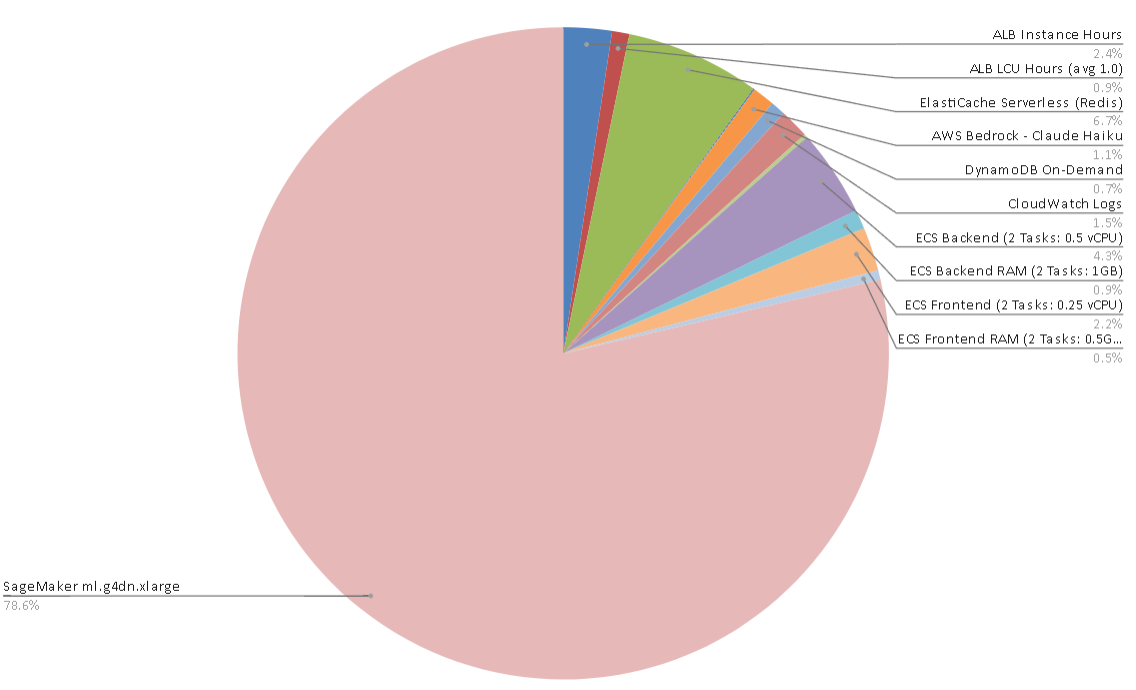
\includegraphics[width=1\textwidth]{img/pdz/31-pie-cost.png}
    \caption[Monthly Cost Breakdown Visualization]{Monthly Cost Breakdown Visualization (50 Users).}
    \label{fig:monthly_cost_pie}
\end{figure}

\newpage

The following table provides a comparative analysis of GPU operational costs across different cloud providers. This estimation is based on a workload scenario of 50 active users, with each user initiating 20 requests per day and each request requiring 15 seconds of GPU inference time, totaling approximately 125 hours of GPU utilization per month.

\begin{table}[H]
    \centering
    \caption{GPU Cost Optimization: AWS vs. Alternatives (50 Users, $\sim$125h GPU/month).}
    \label{tab:gpu_optimization}
    \begin{adjustbox}{max width=\linewidth}
    \begin{tabular}{llllrrr}
        \toprule
        \textbf{Provider} & \textbf{GPU Type} & \textbf{Pricing Model} & \textbf{Pricing Unit} & \textbf{Always-On} & \textbf{50-User Cost} & \textbf{Savings vs AWS} \\
        \midrule
        AWS SageMaker & ml.g4dn.xlarge & Dedicated & \$0.7364 / hr & \$537.57 & \$537.57 & Baseline \\
        RunPod Serverless & NVIDIA T4 & Pay-per-sec & \$0.000164 / s & \$0.00 & \$73.80 & \$463.77 \\
        Modal Labs & NVIDIA T4 & Serverless & \$0.000225 / s & \$0.00 & \$101.25 & \$436.32 \\
        Hyperstack & RTX A4000 & Dedicated & \$0.15 / hr & \$109.50 & \$109.50 & \$428.07 \\
        \bottomrule
    \end{tabular}
    \end{adjustbox}
\end{table}

% \section{Chapter Summary}

% The three dimensions of Phase 2 validation-component-level evaluation, operational performance testing, and cost estimation-converge on a clear assessment: \textbf{BK-MInD is ready for pilot deployment} with identified optimization targets and infrastructure priorities.

% \textbf{Evaluation Dimension (§6.1): Functional Quality Confirmed, Retrieval Identified as Optimization Lever.}

% Document parsing establishes a solid foundation (58.91\% OmniDocBench, 60.98\% DOCX), with exceptional structural fidelity (92.60\% read order) but text-level challenges (47.43\% text score) limiting further gains. Multimodal PDF retrieval shows strong candidate coverage for hybrid text retrieval (93.69\% Recall@10) and stronger top-ranked visual evidence with ColQwen page retrieval (95.66\% Recall@10, 88.91\% nDCG@10). End-to-end RAG validation reveals the system's core strength: 99.5\% faithfulness with zero hallucinations demonstrates reliable grounding, while 72.7\% correctness with 82\% fully-supported answers identifies retrieval precision and chunking depth as the primary optimization targets. Media processing validates across 42 videos with 100\% temporal coverage (16.63\% WER) and near-perfect frame alignment (97.65\%--98.32\%), with OCW generalization confirming robustness across audio sources.

% \textbf{Verdict:} System is \textbf{functionally sound}. Quality pathway forward is clear: improve retrieval depth and chunking strategy to push correctness toward 80\%+.

% \textbf{Testing Dimension (§6.2): Operational Stability Confirmed to 50 Concurrent Users; Indexing Identified as Capacity Bottleneck.}

% Core interactive APIs (authentication, profile, stats) demonstrate zero error rates with sub-2.6s P95 latency at 50 concurrent users. Search and chat streaming remain stable (0\% error, P95 latencies 30.1s and 4.2s respectively), validating the multimodal retrieval and LLM orchestration under load. Background processing (document processing, indexing, media extraction) identifies indexing as the capacity-sensitive workflow: 100\% success at 30 concurrent jobs, 0\% at 40 jobs. This clear boundary enables controlled queue management for production. Frontend performance (PageSpeed Insights) reaches 99/100 desktop and 90/100 mobile, confirming responsive user experience across devices.

% \textbf{Verdict:} System is \textbf{operationally stable for 50-user cohorts}. Capacity management strategy required: strict queue limits on indexing (30 jobs max), autoscaling for worker pools, and batch-write optimization for vector indexes.

% \textbf{Cost Dimension (§6.3): Sustainable Economics at \$683.72/Month for 50 Users; GPU Dominates at 78.62\%.}

% Monthly operational cost for 50 active users totals \$683.72, with SageMaker GPU inference (\$537.57, 78.62\%) dominating the budget. This cost is sustainable for a pilot cohort and scales sub-linearly: GPU utilization is primarily request-dependent, not concurrent-user-dependent. Alternative GPU providers (RunPod Serverless at \$73.80, Hyperstack at \$109.50) offer cost reductions of 86\%--80\%, representing \$428--464 monthly savings if inference latency trade-offs are acceptable. The testing bottleneck (indexing at 30 concurrent jobs) maps to a predictable cost: the 50-user cohort averages approximately 40 documents/day, translating to 15--20 indexing jobs/day, well within safe operating limits without requiring GPU scaling.

% \textbf{Verdict:} System is \textbf{cost-justified for pilot deployment}. Economics improve at scale; GPU cost optimization deferred to Phase 3 post-deployment analysis.

% \noindent\textbf{Production Readiness Statement}

% \vspace{0.3cm}

% \begin{cmt}{Pilot Deployment Authorization}
% BK-MInD achieves \textbf{Beta-grade production readiness}. Component quality is validated (E2E correctness 72.7\%, faithfulness 99.5\%), operational stability confirmed (50 users, 0\% API error rates), and cost model established (\$683.72/month). The system is cleared for \textbf{pilot deployment to an initial student cohort of 20--50 users} with the following gates and improvements:

% \textbf{Deployment Gates (Must-Have):}
% \begin{enumerate}
%     \item Implement strict indexing queue management (max 30 concurrent jobs; queue-based submission for document uploads)
%     \item Configure alerting for key thresholds: search latency > 30s, indexing failure rate > 5\%, API error rate > 1\%
%     \item Establish incident response playbook for common failure modes: indexing timeout, GPU memory exhaustion, Qdrant connection loss
% \end{enumerate}

% \textbf{High-Priority Improvements (Phase 2.5, Pre-Deployment):}
% \begin{enumerate}
%     \item Retrieval optimization: implement cross-encoder reranking for top-5 results (trade 1--2s latency for 2--3\% nDCG gain) to push correctness toward 75\%
%     \item Chunking refinement: experiment with semantic clustering to improve recall@1 from 24\% to 35\%+ for single-answer queries
%     \item Cache optimization: implement Redis caching for popular queries and embedding vectors (potential 30\%+ latency reduction)
% \end{enumerate}

% \textbf{Deferred to Phase 3 (Post-Deployment Analysis):}
% \begin{enumerate}
%     \item Educational effectiveness metrics: conduct formal user study measuring learning gains, study time, feature adoption
%     \item GPU cost optimization: evaluate serverless providers (RunPod, Modal) after validating inference latency and error rates in production
%     \item Scaling strategy: move from dedicated ECS/SageMaker to auto-scaling pools based on observed request patterns
% \end{enumerate}
% \end{cmt}

% \noindent\textbf{Risk Mitigation and Success Criteria}

% \vspace{0.3cm}

% \noindent\textbf{Primary Risks and Mitigations:}

% \begin{table}[H]
%     \centering
%     \caption{Pilot Deployment Risk Matrix.}
%     \label{tab:pilot_risks}
%     \scalebox{0.9}{
%     \begin{tabular}{lp{3.5cm}p{3.5cm}p{4cm}}
%         \toprule
%         \textbf{Risk} & \textbf{Impact} & \textbf{Trigger} & \textbf{Mitigation} \\
%         \midrule
%         Indexing Queue Overload & Failed document processing; user frustration & Indexing jobs > 30 concurrent & Implement queue management; alert at 25 jobs \\
%         Retrieval Latency Spike & Poor search UX; student complaints & Search P95 > 40s & Increase Qdrant replica count; enable query caching \\
%         GPU Memory Exhaustion & Chat/search failures; cascading errors & OOM errors in logs & Reduce batch size; implement request queuing \\
%         Parsing Quality Variance & Silent answer degradation & Correctness drops > 5\% & Implement parsing monitoring per document type \\
%         \bottomrule
%     \end{tabular}
%     }
% \end{table}

% \textbf{Success Criteria for Pilot (Weeks 1--8):}

% \begin{enumerate}
%     \item \textbf{Reliability}: 99.5\%+ uptime; < 1\% error rate on all interactive APIs
%     \item \textbf{Performance}: Search P95 latency < 45s; Chat first-token latency < 5s
%     \item \textbf{Quality}: Maintain 72.7\%+ correctness on synthetic test set; 99\%+ faithfulness (zero hallucinations)
%     \item \textbf{Capacity}: Sustain 30--50 concurrent users without indexing failures; document upload queue < 5 minutes wait time
%     \item \textbf{Cost}: Actual monthly cost within ±10\% of \$683.72 estimate for 50-user cohort
%     \item \textbf{User Adoption}: $\geq$ 80\% of enrolled students engage with at least 3 search/chat interactions in week 1
% \end{enumerate}

% \textbf{Go/No-Go Decision Point (End of Week 1):}

% If success criteria 1, 2, 3, and 5 (reliability, performance, quality, cost) are met, proceed to full pilot. If any fails, apply targeted fixes before proceeding.

\newpage
